\documentclass[11pt]{article}

\usepackage{titlesec}
\usepackage{graphicx}
\usepackage{caption}
\usepackage{subcaption}
\usepackage{amsmath}
\usepackage{amsfonts}
\usepackage{amssymb}
\usepackage{hyperref}
\usepackage{enumitem}
\usepackage{listings}
\usepackage{xcolor}

% Define colors for syntax highlighting
\definecolor{mygreen}{rgb}{0,0.6,0}
\definecolor{mygray}{rgb}{0.5,0.5,0.5}
\definecolor{mymauve}{rgb}{0.58,0,0.82}

% Set up the MATLAB code listing style
\lstset{
  backgroundcolor=\color{white},
  basicstyle=\footnotesize\ttfamily,
  breakatwhitespace=false,
  breaklines=true,
  captionpos=b,
  commentstyle=\color{mygreen},
  deletekeywords={...},
  escapeinside={\%*}{*)},
  extendedchars=true,
  frame=single,
  keepspaces=true,
  keywordstyle=\color{blue},
  language=Matlab,
  otherkeywords={*,...},
  numbers=left,
  numbersep=5pt,
  numberstyle=\tiny\color{mygray},
  rulecolor=\color{black},
  showspaces=false,
  showstringspaces=false,
  showtabs=false,
  stepnumber=1,
  stringstyle=\color{mymauve},
  tabsize=2,
  title=\lstname
}


% Adjust the margins if needed
\usepackage[left=1in, right=1in, top=1in, bottom=1in]{geometry}
\usepackage{graphicx}
\usepackage{graphicx}
\usepackage{tabto}

% Set the title and author
\title{Iteration and Error}
\author{David Tran and Spencer Kelly}
\date{\today}

\begin{document}

\maketitle

\subsection*{Abstract}
The following series of labs explore different algorithms in numerical analysis, as well as their applications. We offer an exploratory look on each of the algorithms, including notes on its implementation, properties of the algorithms, and the practical effects of its implementation on real-world systems.

This lab introduces the concept of iteration in numerical algorithms through use of Taylor series. Through computations, we show how well the Taylor series approximates a function, and additionally quantify the error in its approximation. We observe and discuss the effects of truncation and precision or rounding errors which occur due to the limitations of hardware, and show how we can measure and differentiate between the two.

\subsection*{Introduction}
In the field of numerical analysis, one of the first important concepts introduced is the idea of approximating otherwise complex and computationally expensive to evaluate functions using much simpler and efficient methods.
In this lab, the first of four, we delve into the approximations of functions using their Taylor series and their associated Taylor remainders, exposing the reader to introductory concepts in functional approximation.

Taylor series are a powerful tool in mathematics, and provide us with a means of representing a smooth function using an infinite series of polynomial terms.
These series allow us to work with otherwise difficult functions, and have applications in a variety of fields including physics, engineering, and quantitative finance, where they aid in modeling complex systems, solving differential equations, and the analysis of complex functions, to name a few.

For the purposes of computation, it is not realistic to use the infinite taylor series for a given function.
In this lab, we introduce the truncated (finite terms) Taylor series for a single function.
We will compare the truncated Taylor series to the function in which it approximates, and analyze the difference between the two, over various domains.
We will also analyze the Taylor remainder, which represents the error associated with truncation to finite terms.
By analyzing the differing number of terms before truncation and plotting the Taylor remainder, we can observe how the degree of truncation effects the accuracy of the approximation, providing insight into the tradeoff between efficiency and accuracy in the field of numerical analysis.

The field of numerical analysis in some form dates back over 2000 years ago in ancient Egypt, and there is evidence to suggest that Babylonians may have used numerical methods to calculate the square root of 2 to within 5 decimal places.
Though using more modern methods, and with the help of the computational software MATLAB, this lab serves as an introduction to methods of computation and approximation in numerical analysis that have been of great use across many fields and civilizations.

\section{Taylor series and error}

\setcounter{subsection}{-1}
\subsection{Problem 0}
Let $f(x) = e^{-x}$. Note that $f^{(1)}(x) = -e^{-x}, f^{(2)}(x) = e^{-x}$, and in general, $f^{(n)}(x) = (-1)^ne^{-x}$. So, $f^{(n)}(0) = (-1)^n$, and the Taylor series expansion around $x_0 = 0$ is given by

\begin{align*}
T_n(x) &= \sum_{k = 0}^n \frac{f^{(k)}(x_0)}{k!} x^k \\
&= \sum_{k = 0}^n \frac{(-1)^k}{k!}x^k
\end{align*}

Similarily, the remainder term is

\begin{align*}
R_n &= \frac{f^{(n + 1)}(z)}{(n + 1)!}(x - x_0)^{n + 1} \\
&= \frac{(-1)^{n + 1} e^{-c}}{(n + 1)!}x^{n + 1}.
\end{align*}

for some $0 \leq c \leq x$.

\subsection{Problem 1}
\begin{enumerate}[label=\alph*.]
  \item We have \begin{align*}
    e^{-x} &= 1 - x + \frac{x^2}{2!} - \frac{x^3}{3!} + \dots
  \end{align*}
  so
  \begin{align*}
    F(x) &= \frac{e^{-x} - 1 + x}{x^2} \\
    &= \frac{1}{2!} - \frac{x}{3!} + \frac{x^2}{4!} - \dots \\
    &= \sum_{k = 0}^\infty (-1)^k \frac{x^k}{(k + 2)!}
  \end{align*}

  and its Taylor series up to $n + 1$ terms is

  $$
  T_n(x) = \sum_{k = 0}^n (-1)^k \frac{x^k}{(k + 2)}
  $$

  To find the remainder term $R_n$, we use the fact that $R_n = F(x) - T_n(x)$. 
  \item We know that the Taylor remainder is in general written as
  $$\frac{f^{k+1}(c)}{(k+1)!}(x-x_0)^{k+1}$$

 So that, in this case, we end up with our taylor series of $n+1$ terms having remainder term:
 $$\frac{(-1)^{n+1}}{((n+1)+2)!}(x)^{n+1} = \frac{(-1)^{n+1}}{(n+3)!}(x)^{n+1}$$

 This tells us that the bound for the truncation error can be written as

 $$\frac{(|x|)^{n+1}}{((n+1)+2)!}$$
\end{enumerate}

\subsection{Problem 2}
We compute and plot $F(x)$ from above with the following.
  
  \lstinputlisting{FTaylor.m}

  \lstinputlisting{plotF.m}

giving the graph in Figure~\ref{fig:lab1b_2}:

\begin{figure}[h!]
  \centering
  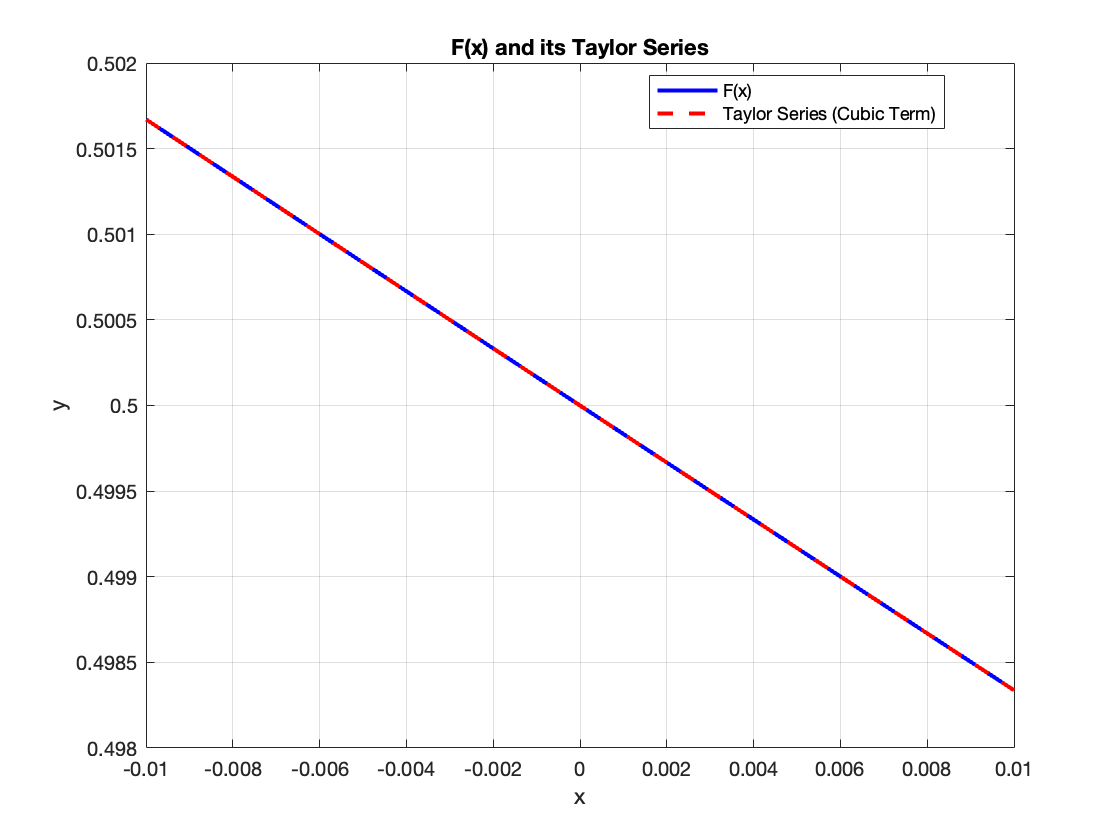
\includegraphics[width=0.8\linewidth]{lab1b_2.png}
  \caption{$F(x)$ and its Taylor Series from $(-0.01, 0.01)$}
  \label{fig:lab1b_2}
\end{figure}

\subsection{Problem 3}

Plotting the graph from Problem 2 using instead a range of $(-10^{-7}, 10^{-7})$ yields Figure~\ref{fig:lab1b_3}. Observe the absolute and relative errors over the interval $(-10^{-6}, 10^{-6})$ in Figure~\ref{fig:lab1b_3_error}. We use the truncation error term in Problem 1 as an upper bound on truncation error. If we plot this alongside the absolute and relative errors as in Figure~\ref{fig:lab1b_3_error_bound}, we see the absolute and relative errors are well above the theoretical truncation error. Also note that the truncation error decreases as we approach 0 and increases as we move away from it, since our Taylor series expansion is centered at $x = 0$. Because the absolute and relative errors are above the truncation error, the problem is roundoff error rather than truncation error. This is because the order of magnitude of the values we are working with ($10^[-6]$) are so small that we approach the machine epsilon when we take powers of these values. The limited precision of floating-point numbers mean that we can't represent these values as precisely. Indeed, as we get small enough, we can \textit{underflow}: where the number is smaller than our floating-point representation can represent. This lack of floating-point precision is what is making the roundoff errors so large.

So, the directly computed function is more accurate. We know the closed form of $F(x)$, so we should use it, rather than approximate the function with the terms of a Taylor series, since, at values of such a small magnitude, it introduces more roundoff error.

\begin{figure}[h!]
  \centering
  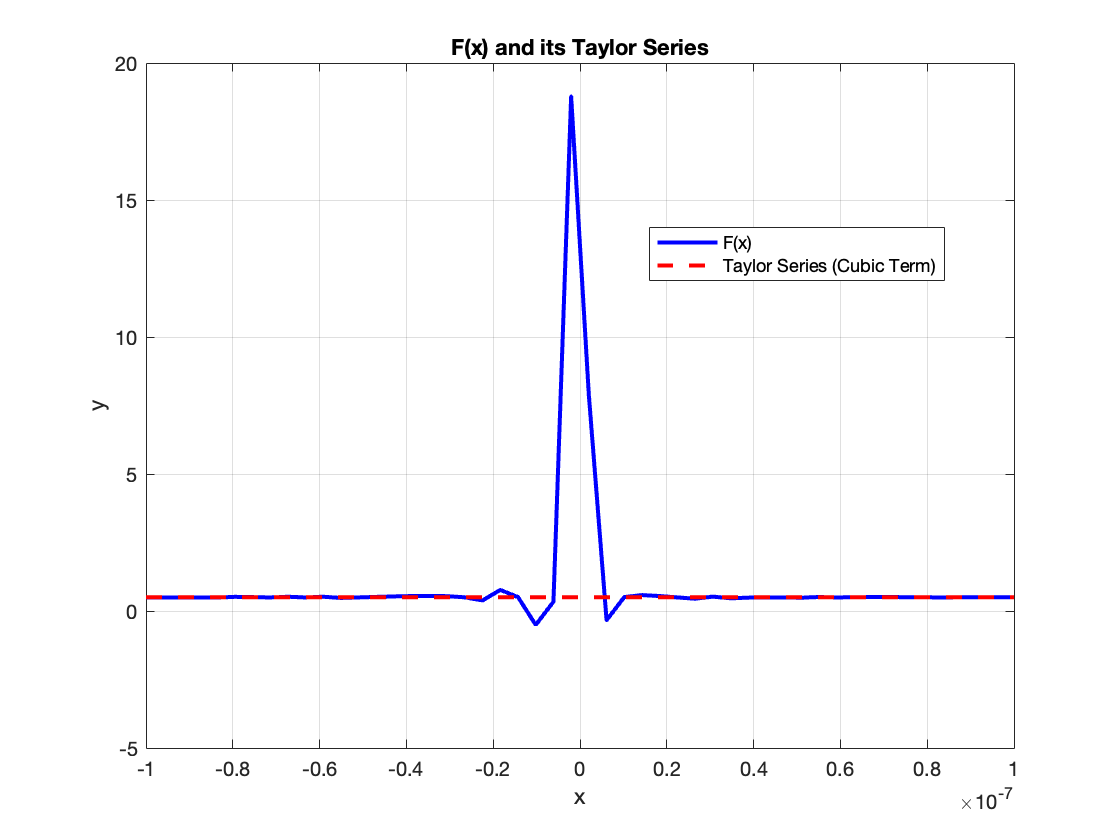
\includegraphics[width=0.8\linewidth]{lab1b_3.png}
  \caption{$F(x)$ and its Taylor Series from $(-10^{-7}, 10^{-7})$ up to cubic terms}
  \label{fig:lab1b_3}
\end{figure}

\begin{figure}[h!]
  \centering
  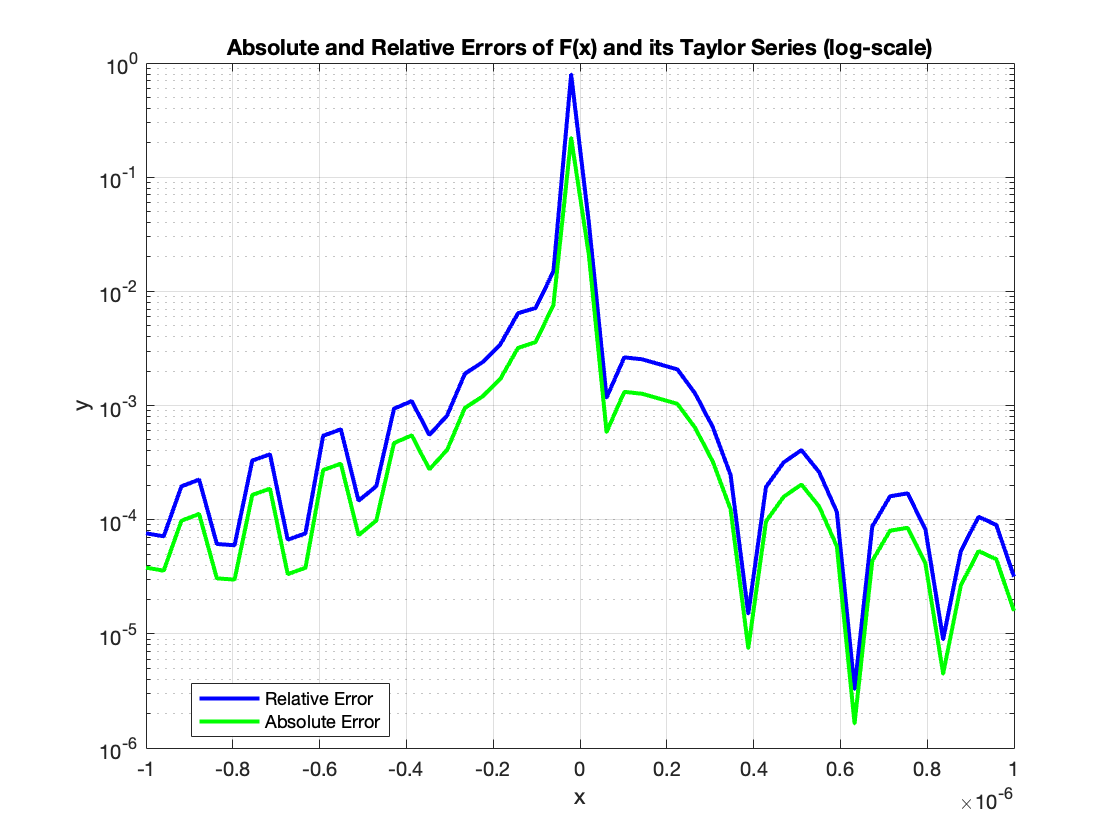
\includegraphics[width=0.8\linewidth]{lab1b_3_error.png}
  \caption{Error between $F(x)$ and its Taylor Series}
  \label{fig:lab1b_3_error}
\end{figure}

\begin{figure}[h!]
  \centering
  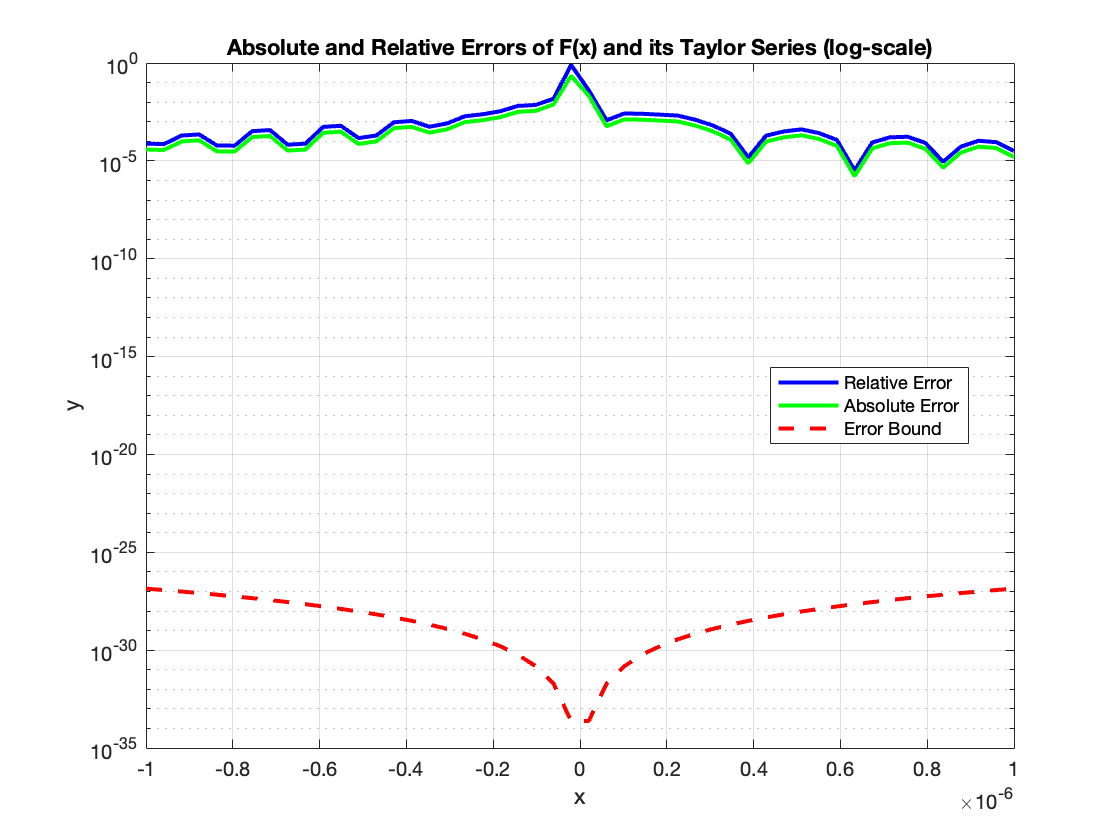
\includegraphics[width=0.8\linewidth]{lab1b_3_error_bound.png}
  \caption{Error between $F(x)$ and its Taylor Series and truncation bound}
  \label{fig:lab1b_3_error_bound}
\end{figure}

\subsection{Problem 4}
Below in Figure~\ref{fig:q41} is the plot of the domain from problem 2 done using the function myfofxv2.m, which uses a taylor series expansion
to plot x values between $-10^{-7}$ and $10^{-7}$. If the value falls not between those bounds, then the functions opts for the original form of the function.

\begin{figure}[h!]
\centering
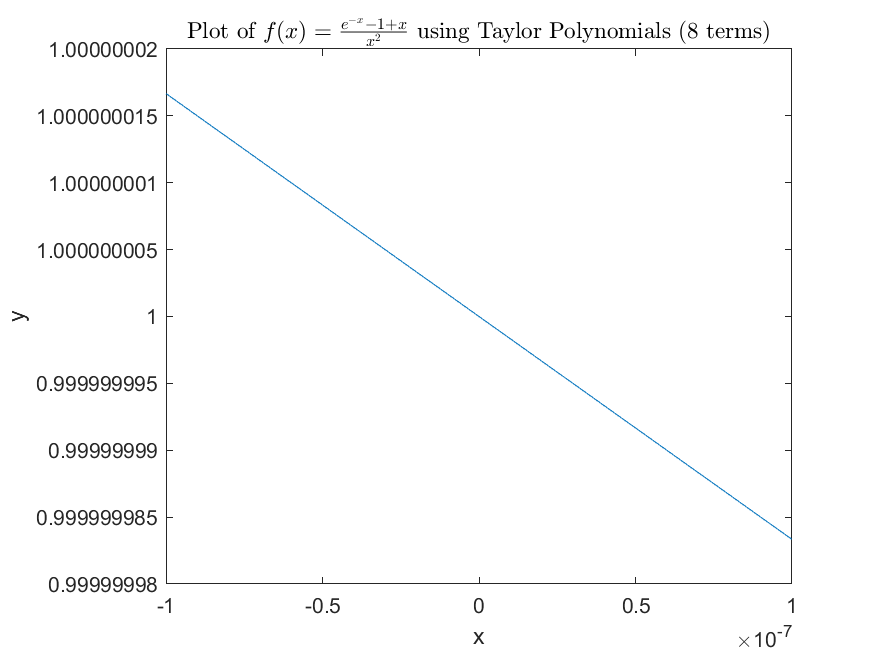
\includegraphics[width=\linewidth]{Lab1BQ4p1q2.png}  % Adjust the file name and extension
\caption{Plot of domain from Problem 2}
\label{fig:q41}
\end{figure}

Below in Figure~\ref{fig:q42} is the plot of the domain from problem 3, using the same function:

\begin{figure}[h!]
\centering
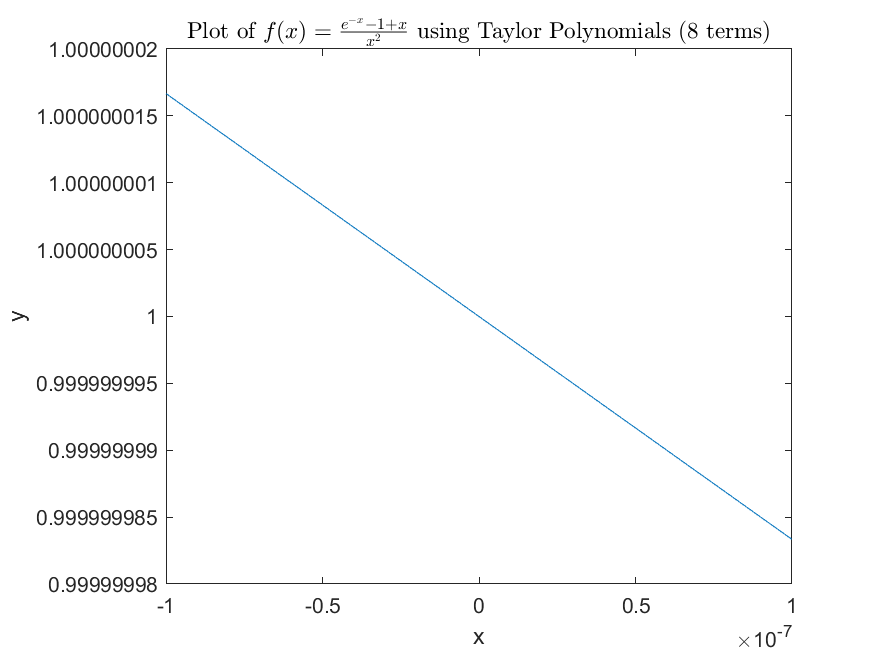
\includegraphics[width=\linewidth]{Lab1BQ4p1q3.png}  % Adjust the file name and extension
\caption{Plot of domain from Problem 3}
\label{fig:q42}
\end{figure}


\section{Summary and Conclusions}

In this lab, we used the Taylor series the approximate a function whose closed-form we knew. We plotted the approximation alongside the closed form to observe how well the Taylor series was able to approximate, as well as where it fell short. We found both analytically and empirically the expected error due to truncation of the series, and discovered that roundoff errors dominated the error over truncation errors at very small values of $x$.

The method of using a Taylor series to approximate a function is very applicable and often used to compute values for functions whose closed form we do not know. For example, in many programming languages, the trigonometric functions are defined in terms of their power series, and 3 to 4 terms are usually used as enough to achieve the maximum-allowed precision due to floating-point representation. For future work, it wouuld be good to explore the threshold at which roundoff error begins to dominate truncation error, as well as discover possible workarounds for approximating functions with Taylor series at very small input values.

\section*{Teamwork Statement}
There were minimal issues encountered as we worked on this lab as a team.
Both lab members were well-equipped with knowledge on the theory pertaining to Taylor series and their applications.
Lab members were also experienced with the applications of Taylor series, and had experience with projects on numerical methods and their applications to other fields of work including modelling of stellar atmospheres, modelling of thermodynamic and electromagnetic systems, and the optimization of algorithms.
Overall, there were little to no problems that arose in terms of teamwork on this project.

\clearpage
\section*{Code Appendix}

\lstinputlisting{myfofxv2.m}

\lstinputlisting{plotFTaylorError.m}

\lstinputlisting{myfxv2.m}

\section*{Plot Appendix}

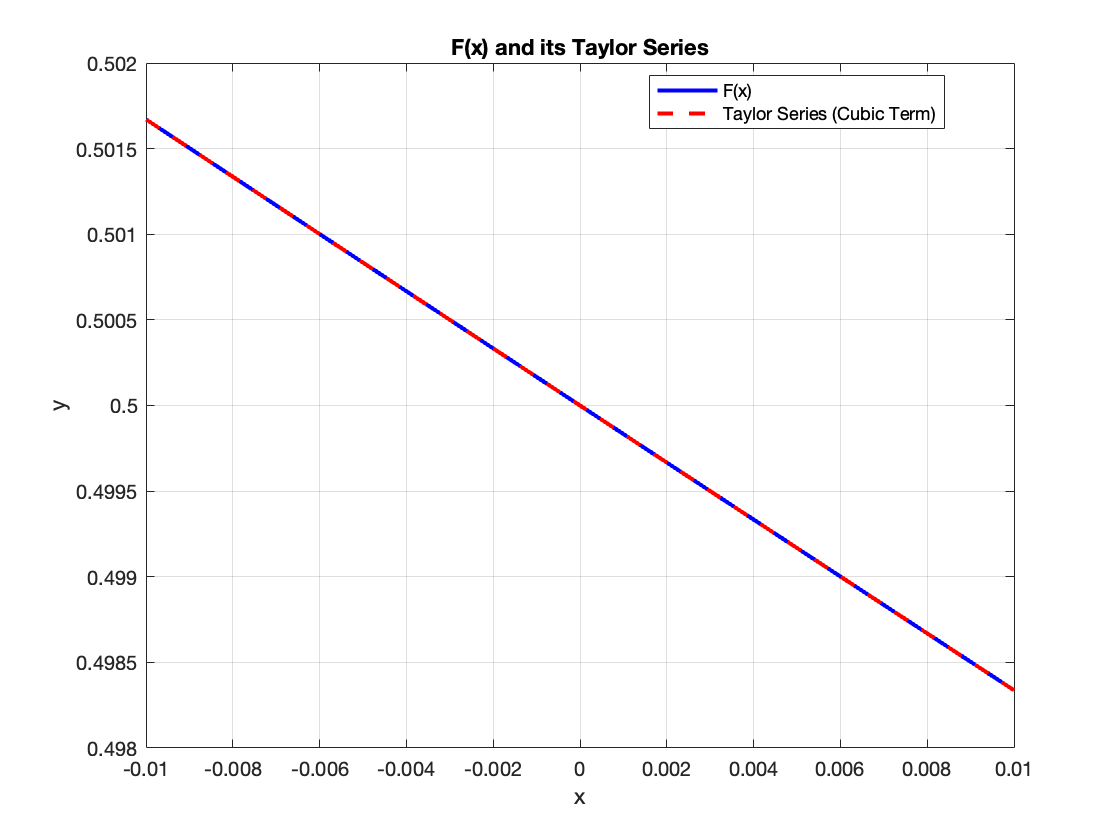
\includegraphics[width=0.8\linewidth]{lab1b_2.png}

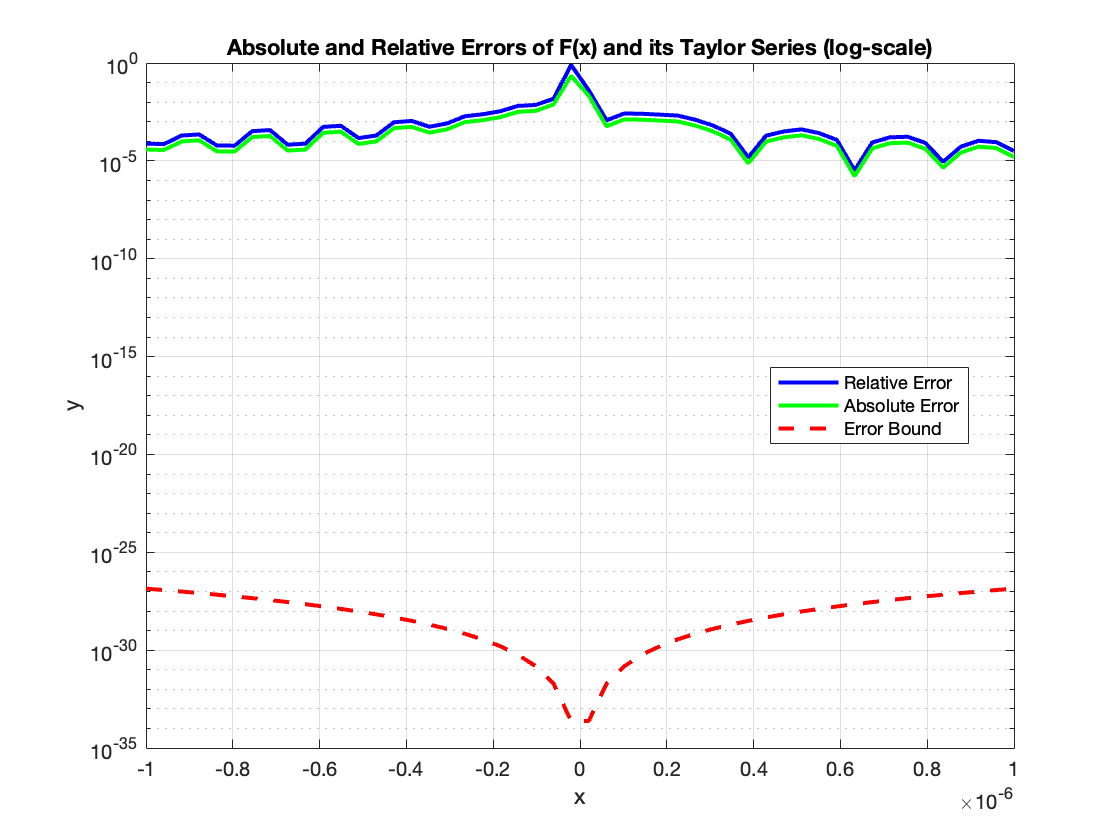
\includegraphics[width=0.8\linewidth]{lab1b_3_error_bound.png}

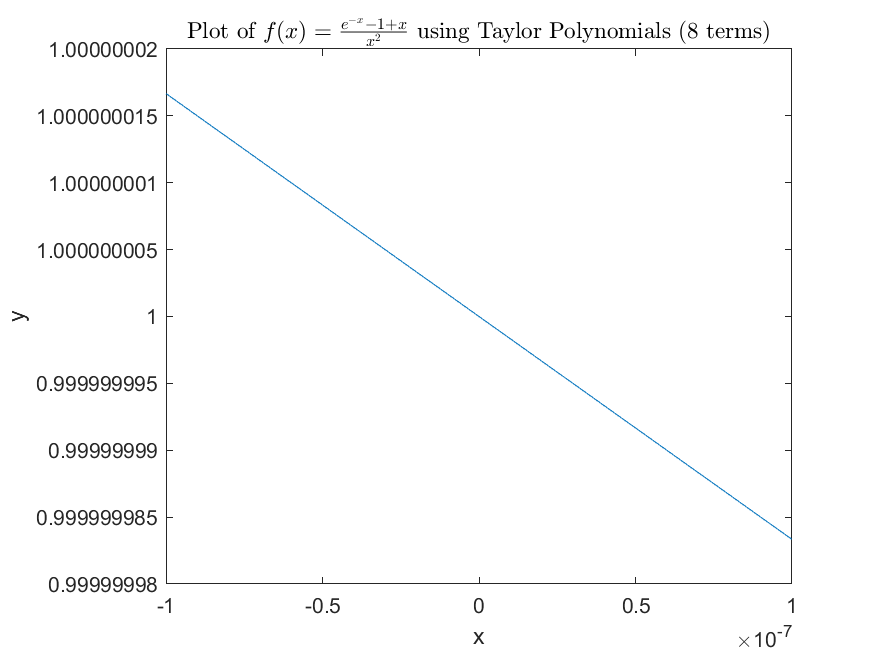
\includegraphics[width=0.8\linewidth]{Lab1BQ4p1q2.png}

\begin{thebibliography}{99}  % Use a number large enough to accommodate the maximum number of references

  \bibitem{britannica}
  Encyclopædia Britannica, inc.
  \newblock \emph{Historical background}.
  \newblock \url{https://www.britannica.com/science/numerical-analysis/Historical-background}.
  
  \bibitem{garcia2015}
  Garcia, A. L.
  \newblock \emph{Numerical Methods for Physics}.
  \newblock CreateSpace, 2015.
  
  \bibitem{leblanc2010}
  Leblanc, F.
  \newblock \emph{An Introduction to Stellar Astrophysics}.
  \newblock John Wiley \& Sons, 2010.
  
  \bibitem{king2010}
  King, G. C.
  \newblock \emph{Vibrations and Waves}.
  \newblock John Wiley \& Sons, 2010.
  
  \bibitem{sauer2019}
  Sauer, T.
  \newblock \emph{Numerical Analysis}.
  \newblock Pearson, 2019.
  
\end{thebibliography}



\end{document}
